% defer/seqlock.tex
% mainfile: ../perfbook.tex
% SPDX-License-Identifier: CC-BY-SA-3.0

\section{Sequence Locks}
\label{sec:defer:Sequence Locks}
%
\epigraph{It'll be just like starting over.}{\emph{John Lennon}}

출간된 시퀀스 락 기록은~\cite{10.1145/800212.806505,10.1145/359863.359878}
reader-writer 락킹의 그것만큼이나 오래 되었습니다만, 시퀀스 락은 상대적으로 덜
알려져 있습니다.
시퀀스 락은 리눅스 커널에서 읽기 쓰레드에게 일관적인 상태로 보여야만 하는
읽기가 대부분인 데이터를 위해 사용됩니다.
하지만, reader-writer 락킹과 달리, 읽기 쓰레드는 쓰기 쓰레드를 배제시키지
않습니다.
그 대신, 해저드 포인터처럼, 시퀀스 락은 읽기 쓰레드가 동시의 쓰기
쓰레드로부터의 활동을 탐지한 경우 오퍼레이션을 \emph{재시도} 하게 합니다.
Figure~\ref{fig:defer:Reader And Uncooperative Sequence Lock}
에서 볼 수 있듯, 읽기 쓰레드들이 아주 가끔만 재시도를 해야 하게끔 코드를
설계하는게 중요합니다.

\iffalse

The published sequence-lock
record~\cite{10.1145/800212.806505,10.1145/359863.359878}
extends back as far as that of reader-writer locking, but sequence locks
nevertheless remain in relative obscurity.
Sequence locks are used in the Linux kernel for read-mostly data that
must be seen in a consistent state by readers.
However, unlike reader-writer locking, readers do not exclude writers.
Instead, like hazard pointers, sequence locks force readers to
\emph{retry} an operation if they detect activity from a concurrent writer.
As can be seen from
Figure~\ref{fig:defer:Reader And Uncooperative Sequence Lock},
it is important to design code using sequence locks so that readers
very rarely need to retry.

\fi

\begin{figure}[tb]
\centering
\resizebox{3in}{!}{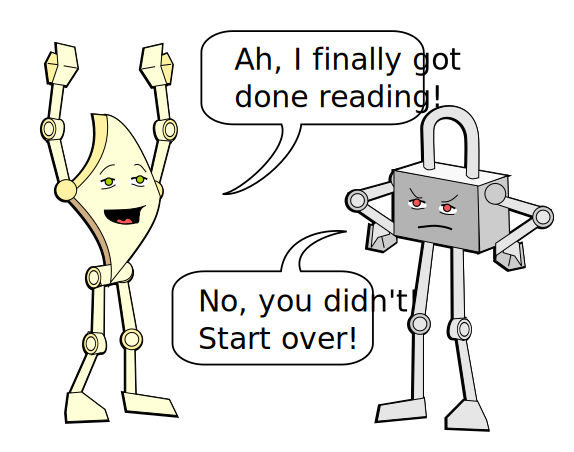
\includegraphics{cartoons/r-2014-Start-over}}
\caption{Reader And Uncooperative Sequence Lock}
\label{fig:defer:Reader And Uncooperative Sequence Lock}
\end{figure}

\QuickQuiz{
	이 시퀀스 락 이야기는 왜 Chapter~\ref{chp:Locking} 에 있지 않죠, 이건
	\emph{락킹} 이잖아요?

	\iffalse

	Why isn't this sequence-lock discussion in Chapter~\ref{chp:Locking},
	you know, the one on \emph{locking}?

	\fi

}\QuickQuizAnswer{
	이 시퀀스 락 메커니즘은 실제로 두개의 별개의 동기화 메커니즘인 시퀀스
	카운트와 락킹의 조합입니다.
	사실, 이 시퀀스 카운트 메커니즘은 리눅스 커널에서
	\co{write_seqcount_begin()} 과 \co{write_seqcount_end()} 기능을 통해
	사용할 수 있습니다.

	하지만, \co{write_seqlock()} 과 \co{write_sequnlock()} 의 조합이 리눅스
	커널에서는 훨씬 더 많이 사용됩니다.
	더 중요하게, 많은 사람들이 ``시퀀스 카운트'' 보다는 ``시퀀스 락''
	이라고 말할 때 더 잘 알아들을 겁니다.

	따라서 이 섹션은 사람들이 제목으로부터 이게 무엇인지 이해할 수 있게끔
	``Sequence Locks'' 라고 제목지어져 있으며, ``Deferred Processing'' 으로
	표현되어 있는 이유는 (1) ``시퀀스 락'' 의 ``시퀀스 카운트'' 를 강조하고
	(2) ``시퀀스 락'' 은 간단한 락 그 이상의 무엇이기 때문입니다.

	\iffalse

	The sequence-lock mechanism is really a combination of two
	separate synchronization mechanisms, sequence counts and
	locking.
	In fact, the sequence-count mechanism is available separately
	in the Linux kernel via the
	\co{write_seqcount_begin()} and \co{write_seqcount_end()}
	primitives.

	However, the combined \co{write_seqlock()} and
	\co{write_sequnlock()} primitives are used much more heavily
	in the Linux kernel.
	More importantly, many more people will understand what you
	mean if you say ``sequence lock'' than if you say
	``sequence count''.

	So this section is entitled ``Sequence Locks'' so that people
	will understand what it is about just from the title, and
	it appears in the ``Deferred Processing'' because (1) of the
	emphasis on the ``sequence count'' aspect of ``sequence locks''
	and (2) because a ``sequence lock'' is much more than merely
	a lock.

	\fi

}\QuickQuizEnd

\begin{listing}[bp]
\begin{VerbatimL}
do {
	seq = read_seqbegin(&test_seqlock);
	/* read-side access. */
} while (read_seqretry(&test_seqlock, seq));
\end{VerbatimL}
\caption{Sequence-Locking Reader}
\label{lst:defer:Sequence-Locking Reader}
\end{listing}

\begin{listing}[bp]
\begin{VerbatimL}
write_seqlock(&test_seqlock);
/* Update */
write_sequnlock(&test_seqlock);
\end{VerbatimL}
\caption{Sequence-Locking Writer}
\label{lst:defer:Sequence-Locking Writer}
\end{listing}

시퀀스 락킹의 핵심 컴포넌트는 시퀀스 숫자로, 업데이트 쓰레드가 없을 때에는
짝수가 되며 진행중인 업데이트가 있을 때에는 홀수가 됩니다.
그럼 읽기 쓰레드는 각 액세스 전과 후에 값을 스냅샷 찍어둘 수 있습니다.
두개의 스냅샷 중 어느 하나라도 홀수를 가지고 있다면, 또는 이 두 스냅샷이
다르다면, 동시의 업데이트가 있었다는 말이 되며, 읽기 쓰레드는 이 액세스의
결과를 폐기하고 재시도 해야 합니다.
따라서 읽기 쓰레드는 시퀀스 락으로 보호되는 데이터에 접근할 때
Listing~\ref{lst:defer:Sequence-Locking Reader} 에 보인 \co{read_seqbegin()} 과
\co{read_seqretry()} 함수를 사용해야 합니다.
스기 쓰레드는 각 업데이트 전과 후에 이 값을 증가시켜야만 하고 한번에 하나의
쓰기 쓰레드만이 허용됩니다.
따라서 쓰기 스레드는 시퀀스 락으로 보호되는 데이터를 업데이트 할 때
Listing~\ref{lst:defer:Sequence-Locking Writer} 에 보인 \co{write_seqlock()} 과
\co{write_sequnlock()} 을 사용해야 합니다.

그 결과, 시퀀스 락으로 보호되는 데이터는 임의의 큰 수의 동시 읽기 쓰레드를 가질
수 있지만, 한번에 하나의 쓰기 쓰레드만 가질 수 있습니다.
시퀀스 락킹은 리눅스 커널에서 시간 계측에서 측정 정도를 보호하기 위해
사용됩니다.
시퀀스 락킹은 또한 경로명 순회 중 동시의 이름 변경 오퍼레이션을 감지하기 위해
사용됩니다.

\iffalse

The key component of sequence locking is the sequence number, which has
an even value in the absence of updaters and an odd value if there
is an update in progress.
Readers can then snapshot the value before and after each access.
If either snapshot has an odd value, or if the two snapshots differ,
there has been a concurrent update, and the reader must discard
the results of the access and then retry it.
Readers therefore use the \co{read_seqbegin()} and \co{read_seqretry()}
functions shown in Listing~\ref{lst:defer:Sequence-Locking Reader}
when accessing data protected by a sequence lock.
Writers must increment the value before and after each update,
and only one writer is permitted at a given time.
Writers therefore use the \co{write_seqlock()} and \co{write_sequnlock()}
functions shown in Listing~\ref{lst:defer:Sequence-Locking Writer}
when updating data protected by a sequence lock.

As a result, sequence-lock-protected data can have an arbitrarily
large number of concurrent readers, but only one writer at a time.
Sequence locking is used in the Linux kernel to protect calibration
quantities used for timekeeping.
It is also used in pathname traversal to detect concurrent rename operations.

\fi

\begin{listing}[tb]
\input{CodeSamples/defer/seqlock@impl.fcv}
\caption{Sequence-Locking Implementation}
\label{lst:defer:Sequence-Locking Implementation}
\end{listing}

시퀀스 락의 간단한 구현이
Listing~\ref{lst:defer:Sequence-Locking Implementation}
(\path{seqlock.h}) 에 보여 있습니다.
\begin{fcvref}[ln:defer:seqlock:impl:typedef]
\co{seqlock_t} 데이터 구조는 \clnrefrange{b}{e} 에 보여져 있는데 시퀀스 숫자와
함께 쓰기 쓰레드들을 순서짓기 위한 락을 포함하고 있습니다.
\end{fcvref}
\begin{fcvref}[ln:defer:seqlock:impl:init]
\Clnrefrange{b}{e} 는 이름이 의미하듯 \co{seqlock_t} 를 초기화 하는
\co{seqlock_init()} 를 보입니다.
\end{fcvref}

\begin{fcvref}[ln:defer:seqlock:impl:read_seqbegin]
\Clnrefrange{b}{e} 는 시퀀스 락 읽기 쪽 크리티컬 섹션을 시작하는
\co{read_seqbegin()} 을 보입니다.
라인~\lnref{fetch} 는 시퀀스 카운터의 스냅샷을 취하고, 라인~\lnref{mb} 는 이
호출자의 크리티컬 섹션이 시작되기 전으로 이 스냅샷 오퍼레이션이 순서지어지도록
합니다.
마지막으로, 라인~\lnref{ret} 는 이 스냅샷의 값을 (least-significant bit 이
지워진채로) 리턴하는데, 호출자는 이를 나중의 \co{read_seqretry()} 호출 시에
넘길 겁니다.
\end{fcvref}

\iffalse

A simple implementation of sequence locks is shown in
Listing~\ref{lst:defer:Sequence-Locking Implementation}
(\path{seqlock.h}).
\begin{fcvref}[ln:defer:seqlock:impl:typedef]
The \co{seqlock_t} data structure is shown on
\clnrefrange{b}{e}, and contains
the sequence number along with a lock to serialize writers.
\end{fcvref}
\begin{fcvref}[ln:defer:seqlock:impl:init]
\Clnrefrange{b}{e} show \co{seqlock_init()}, which, as the name indicates,
initializes a \co{seqlock_t}.
\end{fcvref}

\begin{fcvref}[ln:defer:seqlock:impl:read_seqbegin]
\Clnrefrange{b}{e} show \co{read_seqbegin()}, which begins a sequence-lock
read-side critical section.
Line~\lnref{fetch} takes a snapshot of the sequence counter, and
line~\lnref{mb} orders
this snapshot operation before the caller's critical section.
Finally, line~\lnref{ret} returns the value of the snapshot (with the least-significant
bit cleared), which the caller
will pass to a later call to \co{read_seqretry()}.
\end{fcvref}

\fi

\QuickQuiz{
	Listing~\ref{lst:defer:Sequence-Locking Implementation}
	의 \co{read_seqbegin()} 은 왜 이미 망한 읽기가 시작되게 하는 대신
	아래쪽 bit 이 셋 되었는지 검사하고 내부적으로 재시도 하지 않나요?

	\iffalse

	Why not have \co{read_seqbegin()} in
	Listing~\ref{lst:defer:Sequence-Locking Implementation}
	check for the low-order bit being set, and retry
	internally, rather than allowing a doomed read to start?

	\fi

}\QuickQuizAnswer{
	그건 합법적인 구현이 될 겁니다.
	하지만, 워크로드가 읽기가 대부분이라면, 일반적인 경우 성공적 읽기의
	오버헤드를 증가시킬 수 있는데, 이는 생산적이지 못할 겁니다.
	그러나, 충분히 큰 업데이트 쓰레드의 비율과 충분히 높은 읽기 쓰레드의
	오버헤드가 주어진다면, \co{read_seqbegin()} 내부의 체크를 갖는 것이
	선호될 수 있습니다.

	\iffalse

	That would be a legitimate implementation.
	However, if the workload is read-mostly, it would likely
	increase the overhead of the common-case successful read,
	which could be counter-productive.
	However, given a sufficiently large fraction of updates
	and sufficiently high-overhead readers, having the
	check internal to \co{read_seqbegin()} might be preferable.

	\fi

}\QuickQuizEnd

\begin{fcvref}[ln:defer:seqlock:impl:read_seqretry]
\Clnrefrange{b}{e} 는 연관된 \co{read_seqbegin()} 호출 이후 최소 하나의 쓰기
쓰레드가 존재했다면 true 를 리턴하는 \co{read_seqretry()} 를 보입니다.
라인~\lnref{mb} 는 이 호출자의 라인~\lnref{fetch} 의 시퀀스 카운터의 새
스냅샷을 읽어오기 전의 크리티컬 섹션을 순서짓습니다.
라인~\lnref{ret} 는 이 시퀀스 카운터가 변화되었는지 검사하는데, 달리 말하면
최소 하나의 쓰기 쓰레드가 있었는지 검사하고, 그렇다면 true 를 리턴합니다.
\end{fcvref}

\iffalse

\begin{fcvref}[ln:defer:seqlock:impl:read_seqretry]
\Clnrefrange{b}{e} show \co{read_seqretry()}, which returns true if there
was at least one writer since the time of the corresponding
call to \co{read_seqbegin()}.
Line~\lnref{mb} orders the caller's prior critical section before line~\lnref{fetch}'s
fetch of the new snapshot of the sequence counter.
Line~\lnref{ret} checks whether the sequence counter has changed,
in other words, whether there has been at least one writer, and returns
true if so.
\end{fcvref}

\fi

\QuickQuizSeries{%
\QuickQuizB{
	Listing~\ref{lst:defer:Sequence-Locking Implementation} 의
	line~\ref{ln:defer:seqlock:impl:read_seqretry:mb}
	의 \co{smp_mb()} 는 왜 필요한가요?

	\iffalse

	Why is the \co{smp_mb()} on
	line~\ref{ln:defer:seqlock:impl:read_seqretry:mb} of
	Listing~\ref{lst:defer:Sequence-Locking Implementation}
	needed?

	\fi

}\QuickQuizAnswerB{
	그게 없다면, 컴파일러도 CPU 도 \co{read_seqretry()} 앞의 크리티컬
	섹션을 이 함수 다음으로 재배치 할 권리를 갖습니다.
	이는 이 시퀀스 락이 크리티컬 섹션을 보호하는 걸 방해할 겁니다.
	\co{smp_mb()} 기능은 그런 재배치를 막습니다.

	\iffalse

	If it was omitted, both the compiler and the CPU would be
	within their rights to move the critical section preceding
	the call to \co{read_seqretry()} down below this function.
	This would prevent the sequence lock from protecting the
	critical section.
	The \co{smp_mb()} primitive prevents such reordering.

	\fi

}\QuickQuizEndB
%
\QuickQuizM{
	Listing~\ref{lst:defer:Sequence-Locking Implementation}
	의 코드에서는 더 완화된 형태의 메모리 배리어를 사용할 순 없나요?

	\iffalse

	Can't weaker memory barriers be used in the code in
	Listing~\ref{lst:defer:Sequence-Locking Implementation}?

	\fi

}\QuickQuizAnswerM{
	오래전 버전의 리눅스 커널에서는 안됩니다.

	\begin{fcvref}[ln:defer:seqlock:impl]
	매우 최신 버전의 리눅스 커널에서는
	line~\lnref{read_seqbegin:fetch} 은 \co{READ_ONCE()} 대신
	라인~\lnref{read_seqbegin:mb} 의 \co{smp_mb()} 를 없애도 되게 할 수
	있는 \co{smp_load_acquire()} 를 사용할 수도 있습니다.
	비슷하게, 라인~\lnref{write_sequnlock:inc} 는 예를 들면 다음과 같이
	\co{smp_store_release()} 를 사용할 수 있습니다:

	\iffalse

	In older versions of the Linux kernel, no.

	\begin{fcvref}[ln:defer:seqlock:impl]
	In very new versions of the Linux kernel,
        line~\lnref{read_seqbegin:fetch} could use
	\co{smp_load_acquire()} instead of \co{READ_ONCE()}, which
	in turn would allow the \co{smp_mb()} on
        line~\lnref{read_seqbegin:mb} to be dropped.
	Similarly, line~\lnref{write_sequnlock:inc} could use an
        \co{smp_store_release()}, for
	example, as follows:

	\fi

\begin{VerbatimU}
smp_store_release(&slp->seq, READ_ONCE(slp->seq) + 1);
\end{VerbatimU}

	이는 라인~\lnref{write_sequnlock:mb} 의 \co{smp_mb()} 를 제거할 수 있게
	할 겁니다.
	\end{fcvref}

	\iffalse

	This would allow the \co{smp_mb()} on
	line~\lnref{write_sequnlock:mb} to be dropped.
	\end{fcvref}

	\fi

}\QuickQuizEndM
%
\QuickQuizE{
	시퀀스 락킹 업데이트 쓰레드가 읽기 쓰레드를 starve 시키는 걸 무엇이
	방지하나요?

	\iffalse

	What prevents sequence-locking updaters from starving readers?

	\fi

}\QuickQuizAnswerE{
	아무것도요.
	이것은 시퀀스 락킹의 약점 중 하나이며, 그 결과, 여러분은 시퀀스 락킹을
	읽기가 대부분인 환경에서만 사용해야 합니다.
	그렇지 않다면 읽기 쪽의 starvation 은 여러분의 환경에서는 허용되는
	것이니, 이 경우라면, 시퀀스 락킹 업데이트를 가지고 잘 놀아보시기
	바랍니다!

	\iffalse

	Nothing.
	This is one of the weaknesses of sequence locking, and as a
	result, you should use sequence locking only in read-mostly
	situations.
	Unless of course read-side starvation is acceptable in your
	situation, in which case, go wild with the sequence-locking updates!

	\fi

}\QuickQuizEndE
}

\begin{fcvref}[ln:defer:seqlock:impl:write_seqlock]
\Clnrefrange{b}{e} 는 간단히 락을 획득하고 이 시퀀스 숫자를 증가시키며, 이 값
즈가가 이 호출자의 크리티컬 섹션 전으로 순서 지어지게 보장하는 메모리 배리어를
수행하는 \co{write_seqlock()} 을 보입니다.
\end{fcvref}
\begin{fcvref}[ln:defer:seqlock:impl:write_sequnlock]
\Clnrefrange{b}{e} 는 이 호출자의 크리티컬 섹션이 라인~\lnref{inc} 에서의
시퀀스 숫자 증가 전으로 순서 지어지게 하는 메모리 배리어를 수행하고 이 락을
해제하는 \co{write_sequnlock()} 을 보입니다.
\end{fcvref}

\iffalse

\begin{fcvref}[ln:defer:seqlock:impl:write_seqlock]
\Clnrefrange{b}{e} show \co{write_seqlock()}, which simply acquires the lock,
increments the sequence number, and executes a memory barrier to ensure
that this increment is ordered before the caller's critical section.
\end{fcvref}
\begin{fcvref}[ln:defer:seqlock:impl:write_sequnlock]
\Clnrefrange{b}{e} show \co{write_sequnlock()}, which executes a memory barrier
to ensure that the caller's critical section is ordered before the
increment of the sequence number on line~\lnref{inc}, then releases the lock.
\end{fcvref}

\fi

\QuickQuizSeries{%
\QuickQuizB{
	만약 뭔가 다른게 쓰기 쓰레드들을 직렬화 시켜서 이 락이 필요 없게 만들면
	어떤가요?

	\iffalse

	What if something else serializes writers, so that the lock
	is not needed?

	\fi

}\QuickQuizAnswerB{
	이 경우, \co{->lock} 필드는 없어질 수 있는데, 리눅스 커널의
	\co{seqcount_t} 가 그렇습니다.

	\iffalse

	In this case, the \co{->lock} field could be omitted, as it
	is in \co{seqcount_t} in the Linux kernel.

	\fi

}\QuickQuizEndB
%
\QuickQuizE{
	Listing~\ref{lst:defer:Sequence-Locking Implementation} 의
	라인~\ref{ln:defer:seqlock:impl:typedef:seq}
	의 \co{seq} 는 왜 \co{unsigned long} 이 아니라 \co{unsigned} 인가요?
	어쨌건, \co{unsigned} 가 리눅스 커널에 충분히 좋다면, 모두에게도 충분히
	좋아야 하지 않나요?

	\iffalse

	Why isn't \co{seq} on
	line~\ref{ln:defer:seqlock:impl:typedef:seq} of
	Listing~\ref{lst:defer:Sequence-Locking Implementation}
	\co{unsigned} rather than \co{unsigned long}?
	After all, if \co{unsigned} is good enough for the Linux
	kernel, shouldn't it be good enough for everyone?

	\fi

}\QuickQuizAnswerE{
	전혀 그렇지 않습니다.
	리눅스 커널은 다음 순서의 이벤트들을 무시할 수 있게 하는 특별한 속성을
	여럿 가지고 있습니다:
	\begin{enumerate}
	\item	쓰레드~0 이 \co{read_seqbegin()} 을 수행해서,
		line~\ref{ln:defer:seqlock:impl:read_seqbegin:fetch} 에서
		\co{->seq} 를 가져와 그 값이 짝수임을 알게 되고, 따라서
		호출자에게 리턴합니다.
	\item	쓰레드~0 이 자신의 읽기 쪽 크리티컬 섹션을 수행하기 시작하지만
		이어서 오랫동안 preemption 당합니다.
	\item	다른 쓰레드가 반복적으로 \co{write_seqlock()} 와
		\co{write_sequnlock()} 을 호출해서 \co{->seq} 의 값이
		오버플로우 되어 쓰레드~0 이 읽었던 값으로 되돌려집니다.
	\item	쓰레드~0 이 수행을 재개해서, 비일관적인 데이터를 가지고 읽기
		크리티컬 섹션을 완료합니다.
	\item	쓰레드~0 이 \co{read_seqretry()} 를 호출하는데, 이는 쓰레드~0
		이 이 시퀀스 락에 의해 보호되는 데이터의 일관적인 값만을
		보았다고 잘못된 결론을 내립니다.
	\end{enumerate}

	\iffalse

	Not at all.
	The Linux kernel has a number of special attributes that allow
	it to ignore the following sequence of events:
	\begin{enumerate}
	\item	Thread~0 executes \co{read_seqbegin()}, picking up
		\co{->seq} in
		line~\ref{ln:defer:seqlock:impl:read_seqbegin:fetch},
		noting that the value is even,
		and thus returning to the caller.
	\item	Thread~0 starts executing its read-side critical section,
		but is then preempted for a long time.
	\item	Other threads repeatedly invoke \co{write_seqlock()} and
		\co{write_sequnlock()}, until the value of \co{->seq}
		overflows back to the value that Thread~0 fetched.
	\item	Thread~0 resumes execution, completing its read-side
		critical section with inconsistent data.
	\item	Thread~0 invokes \co{read_seqretry()}, which incorrectly
		concludes that Thread~0 has seen a consistent view of
		the data protected by the sequence lock.
	\end{enumerate}

	\fi

	리눅스 커널은 시퀀스 락킹을 가끔만 업데이트 되는 것들을 위해
	사용하는데, 하루 중 시간 정보가 그런 경우입니다.
	이 정보는 최대 밀리세컨드마다 업데이트 되므로, 이 카운터를 오버플로우
	시키려면 7주가 걸립니다.
	만약 어떤 커널 쓰레드가 7주간 preemption 당한다면, 리눅스 커널의
	soft-lockup 코드는 그 동안 매 2분마다 경고를 내보낼 겁니다.

	반대로, 64 비트 카운터에서는 매 \emph{나노}세컨드마다 업데이트가 된다고
	해서 오버플로우를 위해 5세기가 넘게 걸립니다.
	따라서, 이 구현은 64 비트 시스템에서 \co{->seq} 를 위해 64 비트 타입을
	사용합니다.

	\iffalse

	The Linux kernel uses sequence locking for things that are
	updated rarely, with time-of-day information being a case
	in point.
	This information is updated at most once per millisecond,
	so that seven weeks would be required to overflow the counter.
	If a kernel thread was preempted for seven weeks, the Linux
	kernel's soft-lockup code would be emitting warnings every two
	minutes for that entire time.

	In contrast, with a 64-bit counter, more than five centuries
	would be required to overflow, even given an update every
	\emph{nano}second.
	Therefore, this implementation uses a type for \co{->seq}
	that is 64 bits on 64-bit systems.

	\fi

}\QuickQuizEndE
}

\begin{listing}[tbp]
\input{CodeSamples/defer/route_seqlock@lookup.fcv}
\caption{Sequence-Locked Pre-BSD Routing Table Lookup (BUGGY!!!)}
\label{lst:defer:Sequence-Locked Pre-BSD Routing Table Lookup}
\end{listing}

\begin{listing}[tbp]
\input{CodeSamples/defer/route_seqlock@add_del.fcv}
\caption{Sequence-Locked Pre-BSD Routing Table Add\slash Delete (BUGGY!!!)}
\label{lst:defer:Sequence-Locked Pre-BSD Routing Table Add/Delete}
\end{listing}

그래서 시퀀스 락킹이 Pre-BSD 라우팅 테이블에 적용되면 무슨 일이 벌어질까요?
Listing~\ref{lst:defer:Sequence-Locked Pre-BSD Routing Table Lookup}
은 데이터 구조와 \co{route_lookup()} 을,
Listing~\ref{lst:defer:Sequence-Locked Pre-BSD Routing Table Add/Delete}
은 \co{route_add()} 와 \co{route_del()} (\path{route_seqlock.c}) 을 보입니다.
이 구현은 또다시 앞의 섹션에서의 비슷했던 것과 비슷하므로, 차이점만
들여다보겠습니다.

\iffalse

So what happens when sequence locking is applied to the Pre-BSD
routing table?
Listing~\ref{lst:defer:Sequence-Locked Pre-BSD Routing Table Lookup}
shows the data structures and \co{route_lookup()}, and
Listing~\ref{lst:defer:Sequence-Locked Pre-BSD Routing Table Add/Delete}
shows \co{route_add()} and \co{route_del()} (\path{route_seqlock.c}).
This implementation is once again similar to its counterparts in earlier
sections, so only the differences will be highlighted.

\fi

\begin{fcvref}[ln:defer:route_seqlock:lookup]
Listing~\ref{lst:defer:Sequence-Locked Pre-BSD Routing Table Lookup} 에서,
라인~\lnref{struct:re_freed} 는 라인~\lnref{lookup:chk_freed}
와~\lnref{lookup:abort} 에서 검사되는 \co{->re_freed} 를 추가합니다.
라인~\lnref{struct:sl} 은
\end{fcvref}
\begin{fcvref}[ln:defer:route_seqlock:lookup:lookup]
라인~\lnref{goto_retry1}
과~\lnref{goto_retry2} 에서의 라인~\lnref{retry} 의 \co{retry} 라벨로 브랜칭
되고 \co{route_lookup()} 의 라인~\lnref{r_sqbegin}, \lnref{r_sqretry1},
그리고~\lnref{r_sqretry2} 에 의해서 사용되는 시퀀스 락을 추가합니다.
그 영향은 업데이트와 동시에 수행되는 모든 탐색을 재시도 하는 것입니다.
\end{fcvref}

\iffalse

\begin{fcvref}[ln:defer:route_seqlock:lookup]
In
Listing~\ref{lst:defer:Sequence-Locked Pre-BSD Routing Table Lookup},
line~\lnref{struct:re_freed} adds \co{->re_freed}, which is checked on
lines~\lnref{lookup:chk_freed} and~\lnref{lookup:abort}.
Line~\lnref{struct:sl} adds a sequence lock, which is used by \co{route_lookup()}
\end{fcvref}
\begin{fcvref}[ln:defer:route_seqlock:lookup:lookup]
on lines~\lnref{r_sqbegin}, \lnref{r_sqretry1}, and~\lnref{r_sqretry2},
with lines~\lnref{goto_retry1} and~\lnref{goto_retry2} branching back to
the \co{retry} label on line~\lnref{retry}.
The effect is to retry any lookup that runs concurrently with an update.
\end{fcvref}

\fi

\begin{fcvref}[ln:defer:route_seqlock:add_del]
Listing~\ref{lst:defer:Sequence-Locked Pre-BSD Routing Table Add/Delete} 에서,
라인~\lnref{add:w_sqlock}, \lnref{add:w_squnlock}, \lnref{del:w_sqlock},
\lnref{del:w_squnlock1}, 그리고~\lnref{del:w_squnlock2} 는 이 시퀀스 락을 잡고
놓으며, 라인~\lnref{add:clr_freed} 과~\lnref{del:set_freed} 는 \co{->re_freed}
을 다룹니다.
따라서 이 구현은 상당히 단순합니다.
\end{fcvref}

\iffalse

\begin{fcvref}[ln:defer:route_seqlock:add_del]
In
Listing~\ref{lst:defer:Sequence-Locked Pre-BSD Routing Table Add/Delete},
lines~\lnref{add:w_sqlock}, \lnref{add:w_squnlock}, \lnref{del:w_sqlock},
\lnref{del:w_squnlock1}, and~\lnref{del:w_squnlock2}
acquire and release the sequence lock,
while lines~\lnref{add:clr_freed} and~\lnref{del:set_freed} handle \co{->re_freed}.
This implementation is therefore quite straightforward.
\end{fcvref}

\fi

\begin{figure}[tb]
\centering
\resizebox{2.5in}{!}{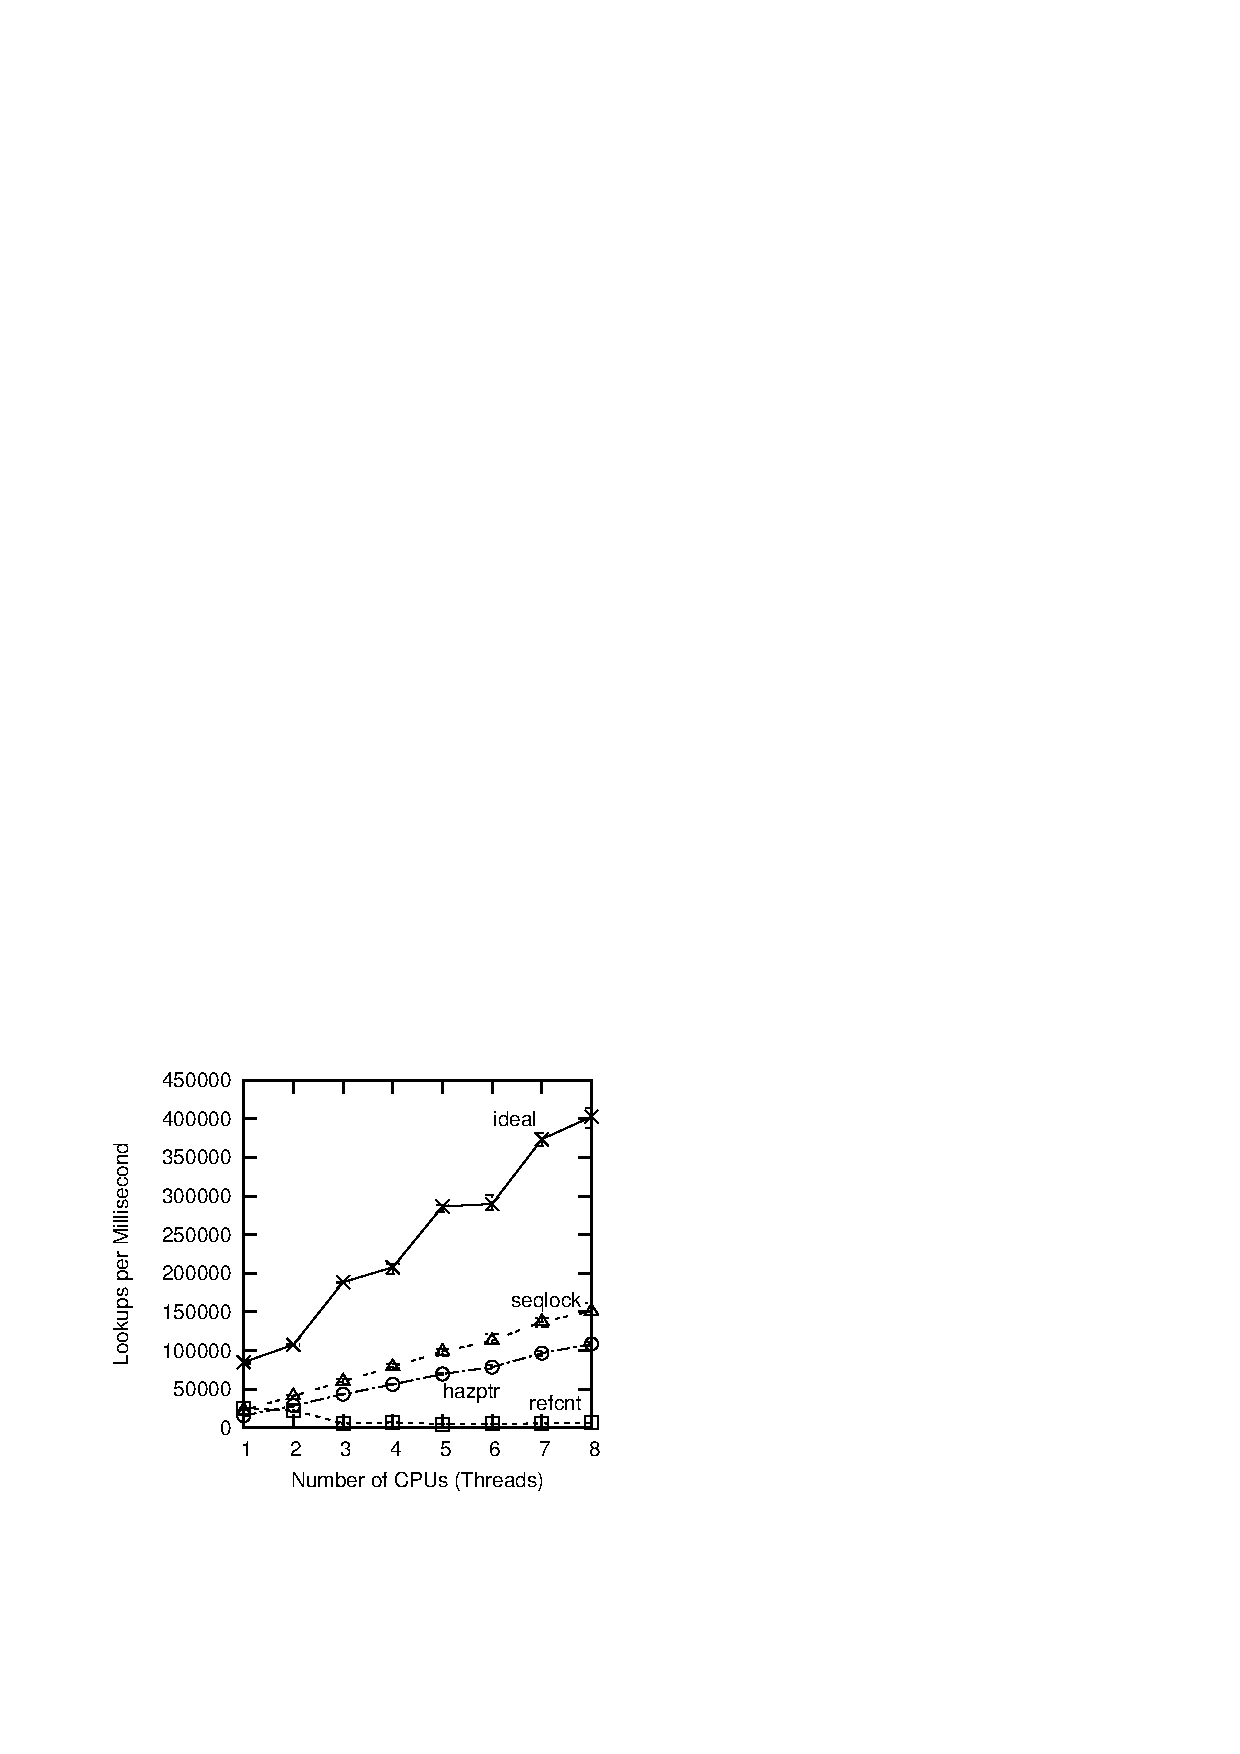
\includegraphics{CodeSamples/defer/perf-seqlock}}
\caption{Pre-BSD Routing Table Protected by Sequence Locking}
\label{fig:defer:Pre-BSD Routing Table Protected by Sequence Locking}
\end{figure}

이것은 또한 읽기 전용 워크로드에서 여전히 이상적인 것에 비해선 떨어지지만 더 잘
성능을 내는데,
Figure~\ref{fig:defer:Pre-BSD Routing Table Protected by Sequence Locking} 에서
이를 볼 수 있습니다.
더 나쁜게, 메모리 해제 후 사용 문제에 취약합니다.
문제는 읽기 쓰레드가 이미 메모리 해제된 구조체를 \co{read_seqretry()} 가 동시의
업데이트를 경고하기 전에 액세스 함으로써 segmentation violation 을 일으킬 수도
있다는 겁니다.

\iffalse

It also performs better on the read-only workload, as can be seen in
Figure~\ref{fig:defer:Pre-BSD Routing Table Protected by Sequence Locking},
though its performance is still far from ideal.
Worse yet, it suffers use-after-free failures.
The problem is that the reader might encounter a segmentation violation
due to accessing an already-freed structure before \co{read_seqretry()}
has a chance to warn of the concurrent update.

\fi

\QuickQuiz{
	이 버그는 고쳐질 수 있나요?
	달리 말하자면, 시퀀스 락을 동시의 추가, 삭제, 그리고 탐색을 지원하는
	링크드 리스트를 보호하는 동기화 메커니즘 \emph{으로만} 시퀀스 락을
	사용할 수 있나요?

	\iffalse

	Can this bug be fixed?
	In other words, can you use sequence locks as the \emph{only}
	synchronization mechanism protecting a linked list supporting
	concurrent addition, deletion, and lookup?

	\fi

}\QuickQuizAnswer{
	이를 이루는 한가지 간단한 방법은 읽기 전용 액세스를 포함한 모든
	액세스를 \co{write_seqlock()} 과 \co{write_sequnlock()} 으로 감싸는
	것입니다.
	물론, 이 해결책은 모든 읽기 쪽의 병렬성을 금지시키기도 해서 상당한 락
	contention 을 초래할 수 있으며, 이는 간단한 락킹을 사용하는
	구현만큼이나 쉬울 겁니다.

	여러분이 읽기 쪽 액세스를 보호하기 위해 \co{read_seqbegin()} 과
	\co{read_seqretry()} 를 사용하는 해결책을 내놓는다면, 여러분이 다음
	순서의 이벤트들을 올바르게 처리함을 분명히 해 두십시오:

	\iffalse

	One trivial way of accomplishing this is to surround all
	accesses, including the read-only accesses, with
	\co{write_seqlock()} and \co{write_sequnlock()}.
	Of course, this solution also prohibits all read-side
	parallelism, resulting in massive lock contention,
	and furthermore could just as easily be implemented
	using simple locking.

	If you do come up with a solution that uses \co{read_seqbegin()}
	and \co{read_seqretry()} to protect read-side accesses, make
	sure that you correctly handle the following sequence of events:

	\fi

	\begin{enumerate}
	\item	CPU~0 이 링크드 리스트를 순회하며, 이 리스트의 원소~A 로의
		포인터를 집어듭니다.
	\item	CPU~1 이 이 리스트로부터 원소~A 를 제거하고 메모리 해제합니다.
	\item	CPU~2 가 연관되지 않은 데이터 구조를 메모리 할당하여, 원소~A 에
		의해 앞서 사용되었던 메모리를 얻게 됩니다.
		이 연관되지 않은 데이터 구조에서, 원소~A 에 의해 \co{->next}
		포인터로 앞서 사용되었던 메모리는 이제 어떤 부동소수점 숫자를
		저장합니다.
	\item	CPU~0 이 원소~A 의 \co{->next} 포인터로 사용되던 것을 집어들어
		무작위적 비트들을 갖게 되고, 따라서 segmentation fault 를
		받습니다.

	\iffalse

	\item	CPU~0 is traversing the linked list, and picks up a pointer
		to list element~A.
	\item	CPU~1 removes element~A from the list and frees it.
	\item	CPU~2 allocates an unrelated data structure, and gets
		the memory formerly occupied by element~A\@.
		In this unrelated data structure, the memory previously
		used for element~A's \co{->next} pointer is now occupied
		by a floating-point number.
	\item	CPU~0 picks up what used to be element~A's \co{->next}
		pointer, gets random bits, and therefore gets a
		segmentation fault.

	\fi

	\end{enumerate}

	이런 종류의 문제로부터의 보호는
	Section~\ref{sec:defer:RCU Provides Type-Safe Memory}
	에서 이야기 될 ``타입-안전 메모리 (type-safe memory'' 를 필요로 합니다.
	대략적으로 비슷한 해결책이
	Section~\ref{sec:defer:Hazard Pointers}
	에서 이야기한 해저드 포인터를 사용하는 비슷한 해결책도 사용 가능합니다.
	그러나 어느 경우든, 여러분은 시퀀스 락에 더해서 어떤 다른 동기화
	메커니즘을 사용해야 할 겁니다!

	\iffalse

	One way to protect against this sort of problem requires use
	of ``type-safe memory'', which will be discussed in
	Section~\ref{sec:defer:RCU Provides Type-Safe Memory}.
	Roughly similar solutions are possible using the hazard pointers
	discussed in
	Section~\ref{sec:defer:Hazard Pointers}.
	But in either case, you would be using some other synchronization
	mechanism in addition to sequence locks!

	\fi

}\QuickQuizEnd

시퀀스 락의 읽기쪽과 쓰기쪽 크리티컬 섹션 모두 트랜잭션들로 생각될 수 있으며,
시퀀스 락킹은 따라서 제한된 형태의,
Section~\ref{sec:future:Transactional Memory} 에서 다룰 트랜잭셔널 메모리
(transactional memory) 로 생각할 수 있습니다.
시퀀스 락킹의 제한점들은: (1)~시퀀스 락킹은 업데이트를 제한하며 (2)~시퀀스
락킹은 업데이트 쓰레드에 의해 메모리 해제될 수도 있는 객체들로의 포인터들을
순회할 수 없습니다.
이 제한들은 물론 트랜잭셔널 메모리에 의해 극복됩니다만 시퀀스 락킹과 다른
동기화 기능들을 조합해서도 극복할 수 있습니다.

\iffalse

Both the read-side and write-side critical sections of a sequence lock
can be thought of as transactions, and sequence locking therefore
can be thought of as a limited form of transactional memory, which
will be discussed in Section~\ref{sec:future:Transactional Memory}.
The limitations of sequence locking are: (1)~Sequence locking restricts
updates and (2)~sequence locking does not permit traversal of pointers
to objects that might be freed by updaters.
These limitations are of course overcome by transactional memory, but
can also be overcome by combining other synchronization primitives
with sequence locking.

\fi

시퀀스 락은 쓰기 쓰레드가 읽기 쓰레드를 뒤로 미뤄지게 할 수 있고, 그 반대도
마찬가지입니다.
이는 unfairness 와 심지어는 쓰기가 많은 워크로드에서의 starvation 을 초래할 수
있습니다.\footnote{
	Dmitry Vyukov 는 읽기 쓰레드 starvation 을 줄일 수 있는 (하지만
	슬프게도 제거할 수는 없는) 한가지 방법을 설명했습니다:
	\url{http://www.1024cores.net/home/lock-free-algorithms/reader-writer-problem/improved-lock-free-seqlock}.}
다른 한편, 쓰기 쓰레드가 없다면, 시퀀스 락 읽기 쓰레드는 합리적 수준으로 빠르고
선형적으로 확장합니다.
두 세계에서 최고를 바라는 건 사람 뿐입니다: 읽기 쪽 실패도, starvation 도
가능하지 않은 빠른 읽기 쓰레드.
또한, 시퀀스 락킹의 포인터에 대한 제약도 극복할 수 있으면 좋을 겁니다.
다음 섹션은 정확히 이런 속성을 가진 동기화 메커니즘을 선보입니다.

\iffalse

Sequence locks allow writers to defer readers, but not vice versa.
This can result in unfairness and even starvation
in writer-heavy workloads.\footnote{
	Dmitry Vyukov describes one way to reduce (but, sadly, not eliminate)
	reader starvation:
	\url{http://www.1024cores.net/home/lock-free-algorithms/reader-writer-problem/improved-lock-free-seqlock}.}
On the other hand, in the absence of writers, sequence-lock readers are
reasonably fast and scale linearly.
It is only human to want the best of both worlds: fast readers without
the possibility of read-side failure, let alone starvation.
In addition, it would also be nice to overcome sequence locking's limitations
with pointers.
The following section presents a synchronization mechanism with exactly
these properties.

\fi
